% IRIS-SIG-13: Mecklenburg-Vorpommern B-Plan Portal Harvester, technical documentation.
% Build:  latexmk -pdf -outdir=build main.tex     (see README.txt)

\documentclass[11pt,a4paper]{article}

% ---------------------------------------------------------------- packages
\usepackage[utf8]{inputenc}
\usepackage[T1]{fontenc}
\usepackage{lmodern}
\usepackage{microtype}
\usepackage[a4paper,margin=2.0cm]{geometry}
\usepackage{booktabs,tabularx,array}
\usepackage{graphicx}
\usepackage{caption}
\usepackage{enumitem}
\usepackage{needspace}
\usepackage{listings}
\usepackage{tikz}
\usetikzlibrary{positioning,shapes.geometric,arrows.meta}
\usepackage[obeyspaces,spaces]{url}   % before hyperref so the options do not clash
\usepackage[hidelinks]{hyperref}

\graphicspath{{../docs/figures/}}

% ---------------------------------------------------------------- layout (plain article)
\setlength{\parindent}{0pt}
\setlength{\parskip}{0.6em}
\setlist{nosep,leftmargin=1.5em,itemsep=0.3em}
\renewcommand{\arraystretch}{1.2}
\captionsetup{font=small,labelfont=bf}

\urlstyle{tt}
% inline code: breaks at slashes and underscores, safe inside tables
\DeclareUrlCommand\codeurl{\urlstyle{tt}}
\newcommand{\code}[1]{{\small\codeurl{#1}}}
\newcommand{\codetxt}[1]{{\small\texttt{#1}}}   % safe in captions and TikZ nodes

\lstset{basicstyle=\ttfamily\small,frame=single,breaklines=true,columns=fullflexible,
  keepspaces=true,aboveskip=0.6em,belowskip=0.4em,showstringspaces=false}

% ---------------------------------------------------------------- title
\title{Mecklenburg-Vorpommern B-Plan Portal Harvester\\[0.3em]
  \large Technical documentation of assignment IRIS-SIG-13}
\author{Arun Kumar Pandey}
\date{\today}

\begin{document}
\maketitle

% ================================================================ 1
\section{Summary}

This document explains how the harvester was built and why it works the way it does. Setup, commands, the file layout
and the list of tests are in the \code{README.md} of the repository, so they are not repeated here. This text covers what
I found at the source, the decisions I made, and how far the result can be trusted.

The brief points to \url{https://b-plan-mv.de}, which no longer exists. I found its successor, the state's
\emph{Bau- und Planungsportal M-V}, and built the harvester on two of its parts: a JSON search service that finds the
plans, and the HTML detail page of each plan, which holds the dates and the document links. The records are loaded into
\code{iris_staging.signal_ingest} as EPSG:25832 points, and running the harvester a second time changes nothing.

\begin{center}
\begin{tabularx}{\textwidth}{@{}>{\bfseries}p{3.6cm}X@{}}
\toprule
Full run, 27 Oct 2026 & 802 distinct candidate plans, of which \textbf{755 solar plans were loaded}. The other 47 matched
 no rule and are listed with their titles. No coordinate had to be rejected.\\
Second run & \code{0 inserted, 0 updated, 755 unchanged}.\\
Not found & No grid landing and no peatland restoration plans. The portal has none (Section~\ref{sec:coverage}).\\
Main caveat & The portal has no publication date, so \code{published_at} is a stand-in (Section~\ref{sec:dates}).\\
\bottomrule
\end{tabularx}
\end{center}

% ================================================================ 2
\Needspace{26\baselineskip}
\section{The acceptance criteria}

The README lists where each deliverable of the brief can be found: the code in \code{src/harvester/}, the tests in
\code{tests/}, the sample output in \code{data/sample/}, the validation queries in \code{sql/02_validation.sql} and
the short error and quality report in \code{docs/quality_report.md}. This is how I read the four acceptance criteria.

\begin{center}
\begin{tabularx}{\textwidth}{@{}>{\raggedright\arraybackslash}p{4.3cm}>{\raggedright\arraybackslash}p{1.5cm}X@{}}
\toprule
\textbf{Criterion} & \textbf{Status} & \textbf{Evidence}\\
\midrule
Right signal types and geographic filtering & Partly &
 The filtering works: every one of the 755 points lies inside the state outline or within 3~km of it, and the titles are on
 topic. But only the solar signal has data, because the portal has nothing for the other two.\\
Valid, traceable records, no duplicates on re-run & Met &
 Every row keeps its source URL, a content hash and the raw record. The second run changed nothing.\\
Errors and missing fields visible, no silent bad coordinates & Met &
 The run report lists every plan that was left out, skipped, rejected or incomplete, with the reason. An impossible
 coordinate rejects the record.\\
Maintainable, configurable, demonstrable offline & Met &
 Rules in a YAML file, settings in \code{.env}, and the whole run can be replayed from saved portal answers.\\
\bottomrule
\end{tabularx}
\end{center}

% ================================================================ 3
\section{The source}\label{sec:source}

\subsection{The URL in the brief}

\url{https://b-plan-mv.de} does not resolve, neither with the local resolver nor with a public one (checked on 27 and
28 October 2026). The brief allows for this case, so I looked for the portal that replaced it.

\subsection{The successor portal}

The state's \emph{Bau- und Planungsportal M-V} lists Bebauungspläne, vorhabenbezogene Bebauungspläne,
Flächennutzungspläne and Satzungen, including plans that are still in preparation. It has three layers, and only two are
useful:

\begin{itemize}
\item The \textbf{HTML listing pages} are empty shells that JavaScript fills in, so there is nothing to read. This is why
  a pure HTML scrape does not work.
\item The \textbf{JSON search service} holds the records. The portal documents it for third parties. I use it to find
  candidates, one query per search term.
\item The \textbf{HTML detail page} of a plan is rendered by the server and is the only place with the dates of the
  legal steps and the document links. I read it for every plan that passes the classification.
\end{itemize}

{\sloppy The search request is
\url{https://www.gaia-mv.de/geoportalsearch/_ajax/search/?type=Bauleitplan&q=<term>&offset=<n>&n=<size>&crs=EPSG:25832},
and a detail page is
\url{https://www.bauportal-mv.de/bauportal/Uebersicht/Details?type=<class>&id=<id>}.\par}

The brief names integration pattern B (HTML). I follow it where it can be followed: the detail pages are read as HTML.
The listing pages cannot be read that way because they are empty, which is why the search goes through the JSON service.

\subsection{What I had to work around}\label{sec:traps}

\begin{enumerate}
\item The counters of the search (\code{total}, \code{hits}, \code{offset}, \code{n}) count result \emph{groups}, not
  records. One plan can appear in several groups, so paging advances by the number of groups received and repeated plans
  are merged afterwards.
\item The search matches inside words. \code{Moor} also finds place names like \emph{Broderstorf}, so the portal's search
  can only collect candidates; the harvester has to decide what is relevant.
\item The centroid comes as \emph{northing,easting}, the reverse of the usual x,y order. The bounding box on the detail
  pages is in EPSG:25833, not 25832, so I do not use it.
\item There is no publication date. The only date in a search record is the time it was indexed. The detail pages have the
  dates of legal steps, and which of them exist depends on the stage of the plan.
\item An unknown plan id returns HTTP 200 with a page that simply has no plan table. A status code alone cannot tell
  that a plan is missing.
\end{enumerate}

\subsection{Access and terms}

I use only the documented interface and public pages, and I bypass nothing. The \code{robots.txt} is a 404 on
\code{bauportal-mv.de} and a 503 page on \code{gaia-mv.de}, so no crawl rules are published, which is not the same as
permission. The harvester therefore identifies itself with a contact address in the \code{User-Agent}, waits two seconds
between requests, retries temporary failures politely and keeps every answer on disk. The portal says the plans belong
to the municipalities and that copying documents needs their consent, so the harvester stores metadata and links only
and downloads no document.

\subsection{What the portal contains}\label{sec:coverage}

Solar plans are plentiful: 755 of them. For the other two signals the portal has nothing. Every \code{Moor} hit is a place
or field name (\emph{Krummes Moor}), the few \code{Umspannwerk} hits are plans next to a substation, and the one
\code{Offshore} hit is a ferry-port extension. A check against the live portal on 28 October 2026, with the grid landing
and peatland terms and an empty cache, took 10 requests, returned 52 records and found no match.

Without the \code{type=Bauleitplan} filter the same search service also returns other GeoPortal content, for example an
offshore cable layer and Moorschutz datasets. Those are map layers and reports, not planning proposals, and I did not
look into them. They may be worth a closer look if the missing signals matter (Section~\ref{sec:open}).

% ================================================================ 4
\section{How it works}\label{sec:design}

\begin{figure}[h]
\centering
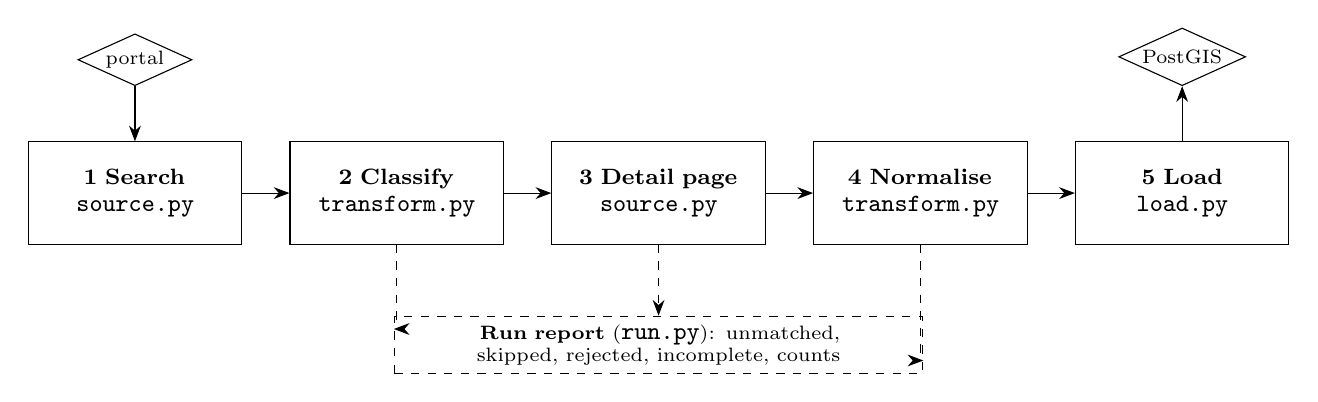
\begin{tikzpicture}[
  node distance=5mm and 6mm,
  box/.style={draw,align=center,font=\footnotesize,minimum height=13mm,text width=2.5cm,inner sep=3pt},
  side/.style={draw,dashed,align=center,font=\scriptsize,text width=6.5cm,inner sep=3pt},
  ext/.style={draw,diamond,aspect=2.2,align=center,font=\scriptsize,inner sep=1pt},
  arr/.style={-{Stealth[length=2mm]}}]
\node[box] (s1) {\textbf{1 Search}\\ \codetxt{source.py}};
\node[box,right=of s1] (s2) {\textbf{2 Classify}\\ \codetxt{transform.py}};
\node[box,right=of s2] (s3) {\textbf{3 Detail page}\\ \codetxt{source.py}};
\node[box,right=of s3] (s4) {\textbf{4 Normalise}\\ \codetxt{transform.py}};
\node[box,right=of s4] (s5) {\textbf{5 Load}\\ \codetxt{load.py}};
\draw[arr] (s1)--(s2); \draw[arr] (s2)--(s3); \draw[arr] (s3)--(s4); \draw[arr] (s4)--(s5);
\node[ext,above=7mm of s1] (portal) {portal};
\node[ext,above=7mm of s5] (db) {PostGIS};
\draw[arr] (portal)--(s1); \draw[arr] (s5)--(db);
\node[side,below=9mm of s3] (rep) {\textbf{Run report} (\codetxt{run.py}): unmatched, skipped, rejected, incomplete, counts};
\draw[arr,dashed] (s2.south) |- ([yshift=2mm]rep.west);
\draw[arr,dashed] (s3.south) -- (rep.north);
\draw[arr,dashed] (s4.south) |- ([yshift=-2mm]rep.east);
\end{tikzpicture}
\caption{One harvest run. Every step that drops a plan writes the reason to the run report.}
\label{fig:pipeline}
\end{figure}

A run searches the portal, keeps the plans that look relevant, reads the page of each of them, cleans the record up and
loads it. Each kept plan becomes one row. It holds the portal's id and the name of the source, the title, the URL of the
plan's page, the links to its documents, the legal status, the kind of plan, the municipality and district as geographic
context, the point, the stand-in publication date and the raw record as received. The 20 columns are described in
\code{docs/data_dictionary.md}. The decisions behind the steps are these.

\textbf{What counts as relevant.} The rules are in \code{config/signals.yaml}: for each of the three signals a list of search
terms and some regular expressions that are applied to the title. Weak words such as \code{Umspannwerk}, \code{Offshore}
or \code{Moor} only count together with a second word, because on their own they mostly mean a place name. The words that
decided are stored with each row, and a plan that matched no rule is listed in the report and never dropped silently.
The price of this approach is that a plan whose title does not name its purpose is missed.

\textbf{Locations.}\label{sec:location} The centroid is swapped to x,y and checked against a box around the state
(10.5 to 14.5\,\textdegree E, 53.0 to 54.8\,\textdegree N). There are three outcomes. If it passes, the point is stored in
EPSG:25832. If the portal gave no centroid, the row is stored without a point and marked \code{unresolved}. If the value
cannot be right, for example degrees instead of metres, the usual x,y order, a point in Poland, \code{0,0} or text, the
record is rejected and reported with the reason, and never loaded. The database enforces the first two cases: a point
exists exactly when the status is \code{resolved}.

\textbf{The publication date.}\label{sec:dates} Since the portal has none, \code{published_at} is the first of these dates
that the detail page has: start of the public display, entry into force, council decision. Which one was used is stored
in \code{raw_payload.published_at_basis} on every row. The first two are dates at which a plan becomes visible to the
public. The council decision comes before any publication, so for 112 rows the column is not really a publication date.
Where the page has no usable date, the column stays empty and the report says so (101 rows). I think this is better than
inventing a date, but it is a decision the users of the data should confirm.

\textbf{Repeating a run.}\label{sec:load} A plan is identified by the portal's own id together with the source name, and the
table has a unique constraint on that pair. For each plan the loader compares a hash of the content with the stored one:
a new plan is inserted, a changed plan is updated in place, and an unchanged plan only gets a new \code{last_seen_at}.
The hash leaves out the raw payload, so a re-run does not look like a change. Every row is written in its own savepoint,
so one row the database refuses does not stop the others. A plan whose detail page could not be read is skipped
completely: loading it without its date and links would overwrite a complete row from an earlier run. Nothing is ever deleted.

\textbf{Failures.}\label{sec:failures} Timeouts, connection errors and HTTP 429 or 5xx are retried after 2, 4 and 8 seconds,
and a \code{Retry-After} header is respected. A search term that keeps failing is reported and the other terms still
run. Empty answers and malformed answers are handled, and a missing detail page, including the ``plan not found'' page,
skips that plan and reports it. If the database is not reachable, the run stops at the start with a one-line message
instead of after a long harvest. The exit code is 0 for a clean run, 2 when something failed that a re-run may fix, and 1
when the run could not start. Each of these cases has a test.

\textbf{Incremental retrieval.}\label{sec:incremental} The portal has no ``changed since'' filter, so every run asks for
everything. This is cheap in practice: all answers are cached on disk, an interrupted run continues where it stopped,
and the upsert writes only what changed.

% ================================================================ 5
\section{Results and data quality}\label{sec:results}

The 786 portal answers of the full run (31 searches and the detail page of each of the 755 kept plans) were fetched on
27 October 2026 and are kept in the repository as a compressed archive with a checksum manifest. The harvester was run
over them offline into an empty database, and then a second time.

\begin{center}
\begin{tabularx}{0.8\textwidth}{@{}Xr@{}}
\toprule
Search records, repeats included & 1,593\\
Distinct candidate records & \textbf{802}\\
Loaded (all solar) & \textbf{755}\\
Matched no rule & 47\\
Rejected for invalid coordinates & 0\\
Skipped for a failed detail page & 0\\
Second run & 0 inserted, 0 updated, 755 unchanged\\
\bottomrule
\end{tabularx}
\end{center}

Of the 47 plans that matched no rule, 40 contain \code{Moor} as a place or field name, 4 are plans next to a substation,
1 is the ferry-port extension, and 2 contain none of these words. None of them is a grid landing or a peatland plan.

The 755 rows are mostly complete. Every row has a point, a municipality, a legal status and a plan type. 101 rows (13\,\%)
have no date because the detail page has none, mostly plans in the draft stage. 98 rows (13\,\%) have no document links
because the municipality has not uploaded any, and one row has no district. The date that stood in for the publication
date was the start of the public display for 319 rows, the entry into force for 223, the council decision for 111 and a
date in a download title for 1. By stage, 319 plans are in force, 427 are in procedure and 9 have ended. One plan has an
entry-into-force date of 31 December 1989, which is implausible for a photovoltaic plan; it is stored as given.

All 755 points lie inside the outline of the state or within 3~km of it. 744 are strictly inside, and the other 11 are at
the coast, where the simplified outline is not exact. None is further out.

\begin{figure}[h]
\centering
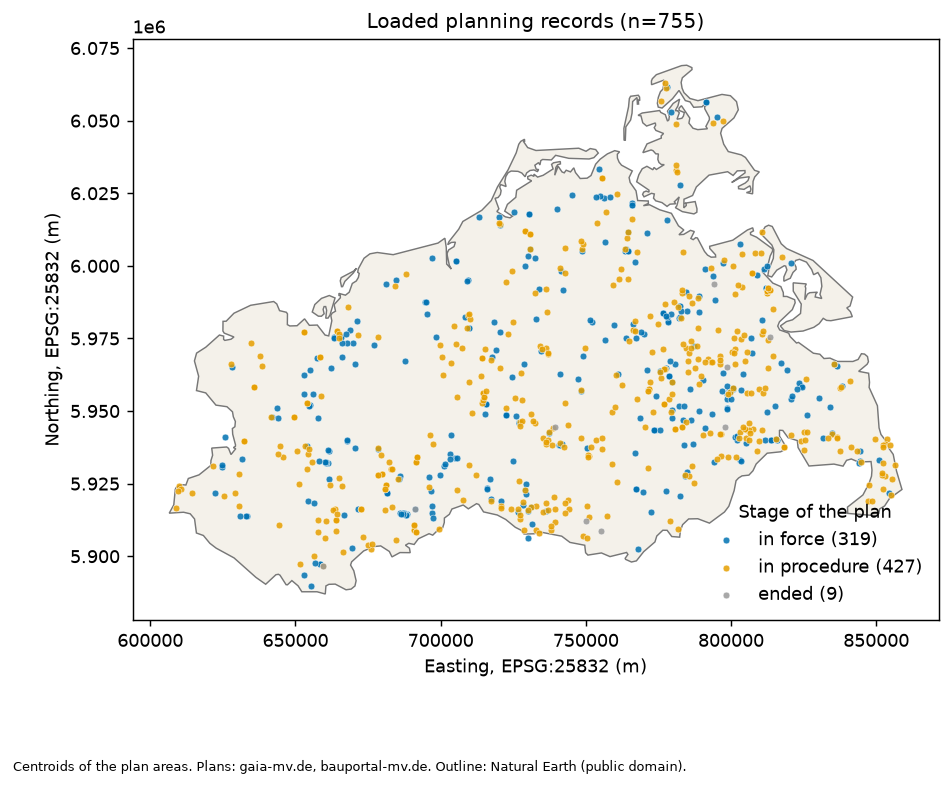
\includegraphics[width=0.72\linewidth]{quicklook}
\caption{The 755 loaded points in EPSG:25832, coloured by stage (quick-look map from \codetxt{qa/quicklook.py}).}
\end{figure}

% ================================================================ 6
\section{Testing and demonstration}\label{sec:tests}

There are 111 automatic tests. HTTP is faked with real saved portal answers (9 search answers and 12 detail pages), so no
test needs the portal. 12 of the tests use PostGIS and run in their own database, so they never touch the rows of a real
run. They cover paging, retries, empty and malformed answers, duplicates, impossible coordinates, and the behaviour of a
re-run: a second load changes nothing, a changed plan is updated in place, and a failed detail page leaves the stored row
alone. The database also has 8 validation queries; each of them must return no rows, and on the loaded data they do. The
tests and the full run were checked on PostgreSQL 16.4 with PostGIS 3.4.3.

\Needspace{9\baselineskip}
Nothing needs access to the portal or to a production system:

\begin{lstlisting}
python tasks.py setup       # environment, local database, raw data
python tasks.py demo        # a small saved sample, loaded twice
python tasks.py test        # the tests
python tasks.py reproduce   # the full run of 755 plans from saved data, then again
python tasks.py validate    # the validation queries
\end{lstlisting}

There are no credentials in the code. Settings come from a \code{.env} file (a template is in the repository), and only a
live run needs the user's own e-mail address, which is sent to the portal in the \code{User-Agent} header.

The README describes these steps in detail, together with the dashboard that shows the table on a map. Python 3.11 or
newer and Docker are needed. I developed and tested on Linux with Python 3.11, 3.12 and 3.13; I have not run it on
Windows or macOS.

% ================================================================ 7
\section{Limitations and open questions}\label{sec:open}

\begin{itemize}
\item Only solar plans were found. The rules and the code for all three signals are in place, but this portal has no
  grid landing or peatland plans that can be told apart from place names.
\item \code{published_at} is a stand-in, and for 112 rows it is the date of the council decision.
\item The signal is decided from the title only.
\item The location check is a bounding box, not the legal state border, and only the centroid of a plan is stored, not its area.
\item Every run is a full refresh, and a cold live run takes half an hour or more because of the pause between requests.
\item The ingestion is a combination of JSON search and HTML detail pages, not a pure HTML scrape, because the HTML
  listing pages are empty.
\end{itemize}

Four questions I would put to the users of the data:
\begin{enumerate}
\item Is another source expected for grid landing and peatland restoration? The same GeoPortal lists related datasets that
  are not planning records.
\item Which date should count as the publication date? The portal has none.
\item Should plans in the draft stage, which have no public date yet, be loaded, or only plans that were made public?
\item Does \code{iris_staging.signal_ingest} already have a defined schema? The brief names the table but no columns, so
  the 20 columns are my own design (see \code{docs/data_dictionary.md}).
\end{enumerate}

\end{document}
